\section{Apresentação Web}
\label{sec:app-web}

Como já mencionado, para apresentação das informações de captura de maneira
acessível foi construida uma aplicação \emph{Web} utilizando as tecnologias
\emph{Node.js}, \emph{MQTT.js}, \emph{html}, \emph{css}, \emph{javascript},
\emph{Bootstrap} e \emph{Google Maps API}.

\emph{Node.js} e a biblioteca de cliente \emph{MQTT.js} foram utilizados para,
da mesma forma exposta no \autoref{code-mqttjs-client}, conectar
uma aplicação escrita em \emph{javascript} com o \emph{MQTT Broker}. Esta
aplicação recupera as informações sobre os dispositos descobertos e as
classifica por proximidade de cada sensor para compor a lista de dispositios
por sensor vista no lado direito da \autoref{fig-web-app}.

Já o \emph{html}, \emph{css}, \emph{javascript} e \emph{Bootstrap} foram
utilizados para estruturar, estilizar, inflar e animar as informações. Em
especial, \emph{Bootstrap} forneceu a estrutura de cabeçalho, rodapé e colulas,
além do esquema de cores.

E a \emph{Google Maps API} juntamente com um pouco de \emph{css} e
\emph{javascript} fornece o mapa visto no lado direito da \autoref{fig-web-app}.
Nele estão reprensentadas as localizações geográficas de cada sensor
representados pelos marcadores nas cores azul e verde.

\begin{figure}[htb]
	\caption{\label{fig-web-app}Web APP}
	\begin{center}
		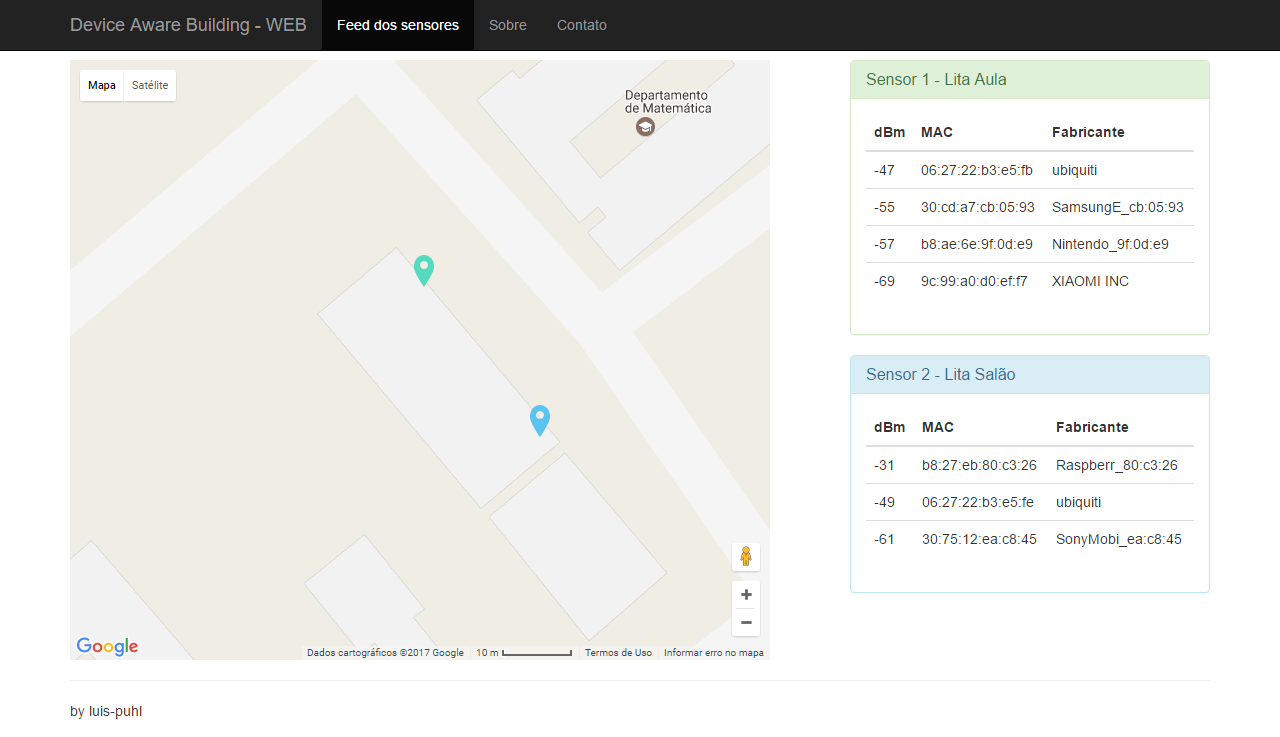
\includegraphics[width=1\textwidth]{050-construcao/web-app.png}
	\end{center}
	\legend{Fonte: Elaborada pelo autor}
\end{figure}
